\documentclass[11pt, a4paper, twoside]{article}   	% use "amsart" instead of "article" for AMSLaTeX format

\usepackage{geometry}                		% See geometry.pdf to learn the layout options. There are lots.
\usepackage{pdfpages}
\usepackage{caption}
\usepackage{minted}
\usepackage[german]{babel}			% this end the next are needed for german umlaute
\usepackage[utf8]{inputenc}
\usepackage{color}
\usepackage{graphicx}
\usepackage{titlesec}
\usepackage{fancyhdr}
\usepackage{lastpage}
\usepackage{hyperref}
\usepackage[autostyle=false, style=english]{csquotes}
\usepackage{mathtools}
\usepackage{tabularx}
% http://www.artofproblemsolving.com/wiki/index.php/LaTeX:Symbols#Operators
% =============================================
% Layout & Colors
% =============================================
\geometry{
   a4paper,
   total={210mm,297mm},
   left=20mm,
   right=20mm,
   top=20mm,
   bottom=30mm
 }	

\definecolor{myred}{rgb}{0.8,0,0}
\definecolor{mygreen}{rgb}{0,0.6,0}
\definecolor{mygray}{rgb}{0.5,0.5,0.5}
\definecolor{mymauve}{rgb}{0.58,0,0.82}

\setcounter{secnumdepth}{4}


% the default java directory structure and the main packages
\newcommand{\srcDir}{../src/}
\newcommand{\imageDir}{./images/}
% =============================================
% Code Settings
% =============================================
\newenvironment{code}{\captionsetup{type=listing}}{}
\newmintedfile[mSourceFile]{matlab}{
	linenos=true, 
	frame=single, 
	breaklines=true, 
	tabsize=2,
	numbersep=5pt,
	xleftmargin=10pt,
	baselinestretch=1,
	fontsize=\footnotesize
}
\newmintinline[mInlineSource]{matlab}{}
\newminted[mSource]{matlab}{
	breaklines=true, 
	tabsize=2,
	autogobble=true,
	breakautoindent=false
}
% =============================================
% Page Style, Footers & Headers, Title
% =============================================
\title{Übung 1}
\author{Thomas Herzog}

\lhead{Übung 1}
\chead{}
\rhead{
\includegraphics[scale=0.10]{FHO_Logo_Students.jpg}}

\lfoot{S1610454013}
\cfoot{}
\rfoot{ \thepage / \pageref{LastPage} }
\renewcommand{\footrulewidth}{0.4pt}
% =============================================
% D O C U M E N T     C O N T E N T
% =============================================
% =============================================
% 2016.10.13: 1 
% 2016.10.14: 2
% =============================================

\pagestyle{fancy}
\begin{document}
\setlength{\headheight}{15mm}
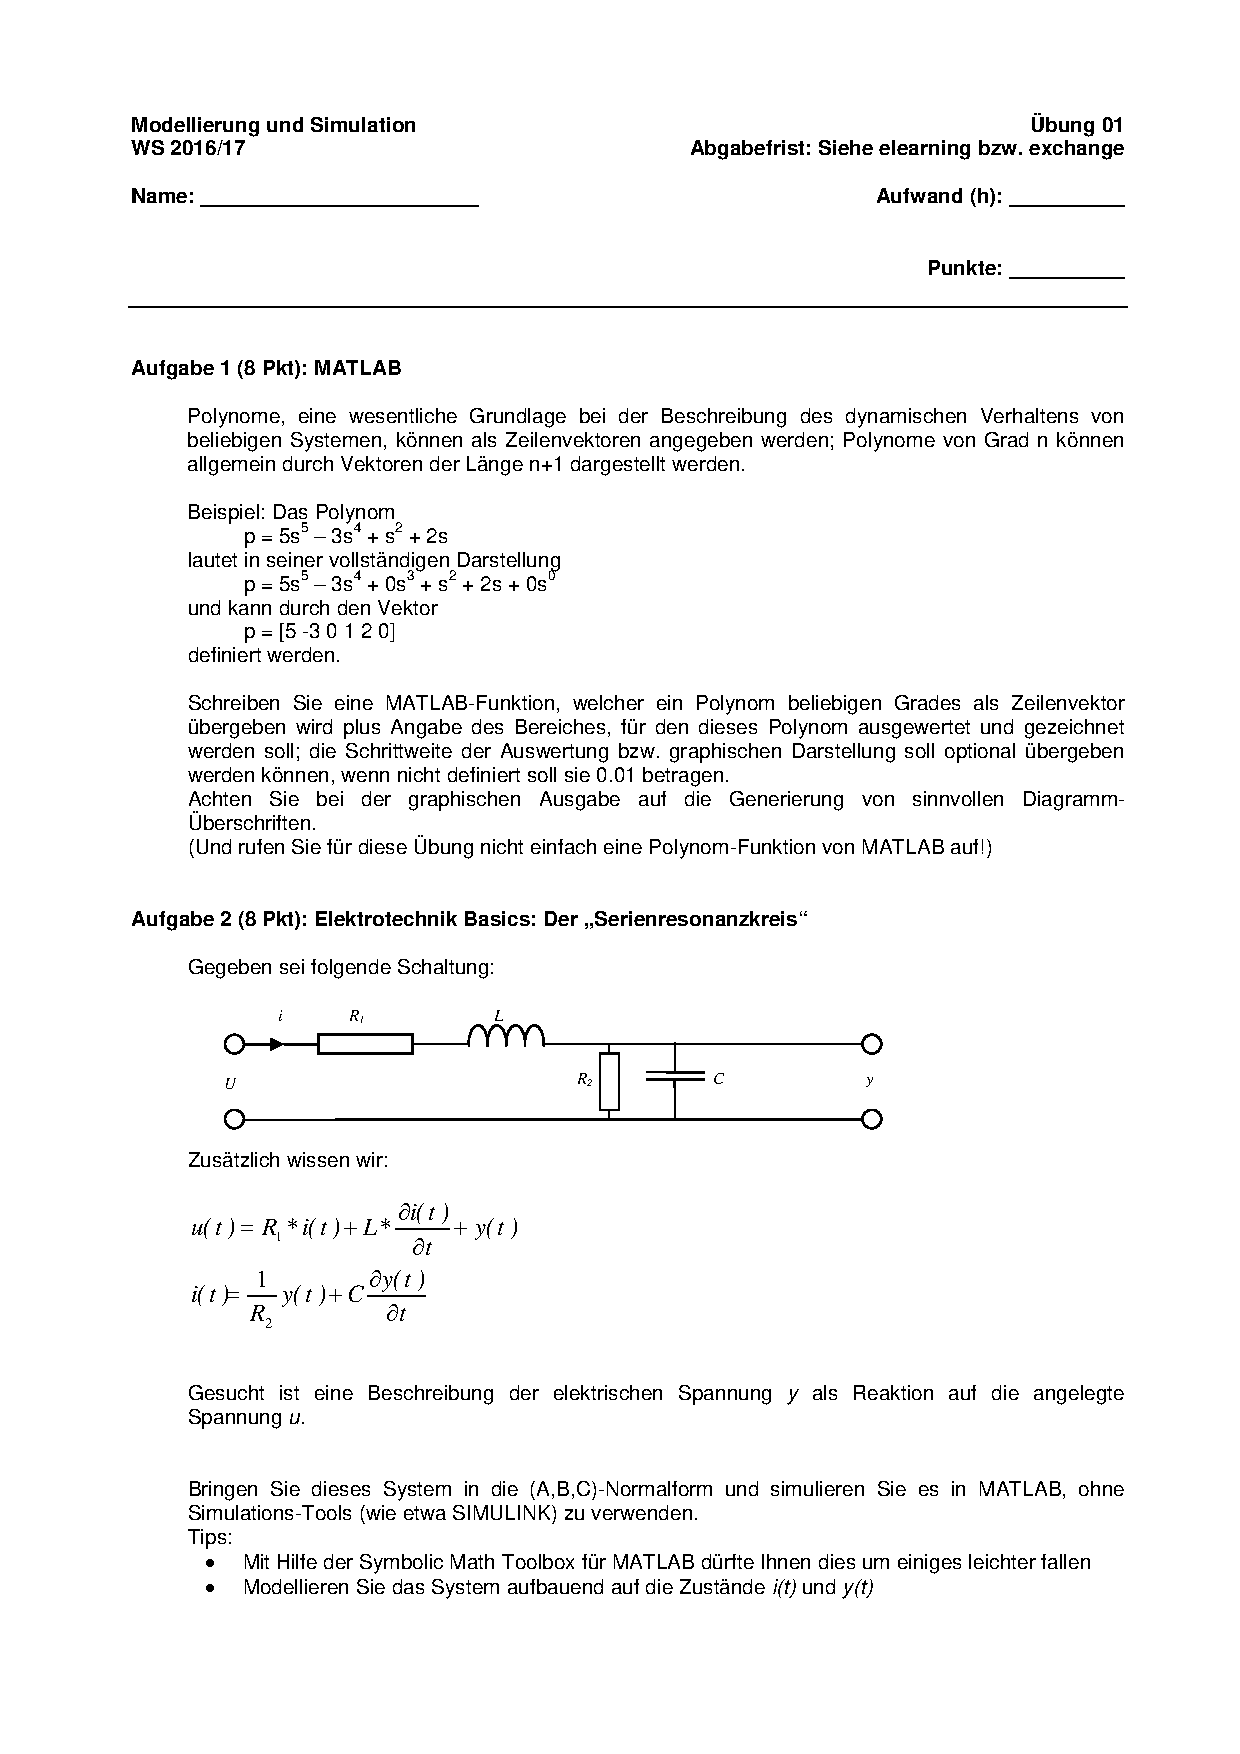
\includepdf[pages={1,2}]{Uebungszettel01.pdf}

% Section gramar and basics 
\section {Matlab}
\label{sec:matlab}
Dieser Abschnitt beschäftigt sich mit der Aufgabenstellung 1 der ersten Übung. Die folgenden Quelltexte zeigen die \emph{Matlab} Funktionen, die für diesen Teil der Übung implementiert wurden.
\newline
\newline
In die Funktion \emph{printPolynom} wurden Prüfungen der übergebenen Argumente implementiert wie
\begin{itemize}
	\item\emph{Gültigkeit der Argumentanzahl}
	\item\emph{Gültigkeit des Vektors}
	\item\emph{Gültigkeit der übergebenen Grenzen und Schrittweite}
\end{itemize}
\ \newline
Wenn die Schrittweite nicht gegeben ist, dann wird der Standardwert $0.01$ verwendet.
\begin{code}
	\caption{Funktion zum Plotten eines Polynoms des Grades n}
	\mSourceFile{\srcDir/printPolynom.m}
\end{code}
\begin{code}
	\caption{Funktion zum Umwandeln eines Polynoms des Grades n in eine Zeichenklette}
	\mSourceFile{\srcDir/poly2Str.m}
	\label{fig:print-poly}
\end{code}
\ \newline
Die Funktion aus dem Quelltext \ref{fig:print-poly} zeigt die Funktion, die implementiert wurde, um die Polynomfunktion repräsentiert durch einen Zeilenvektor in seine Repräsentation mit einer Zeichenkette zu konvertieren. Dies war erforderlich, da die Funktion \emph{poly2Sym} nicht zur Verfügung stand.
\newpage
\subsection{Simulation des Polynoms}
Folgender Abschnitt beschäftigt sich mit den Simulationen des Polynoms.
\newline
\begin{figure}[h]
\centering
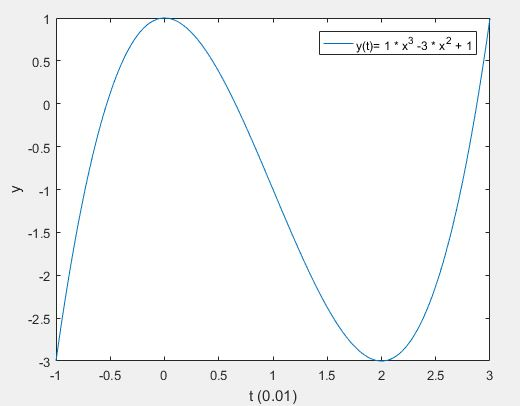
\includegraphics[scale=0.75]{\imageDir/sim_poly_0.JPG}
\caption{Simulation 1 P=[1 -3 0 1]}
\label{fig:sim-resonance-01}
\end{figure}

\begin{figure}[h]
\centering
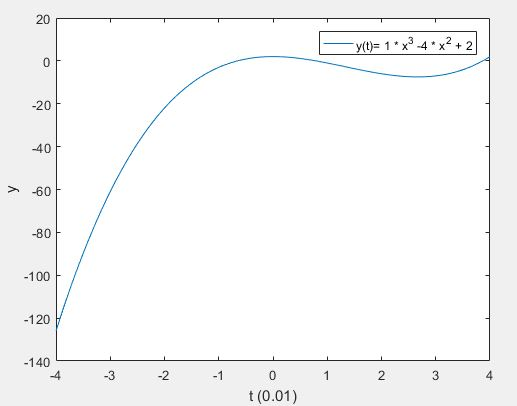
\includegraphics[scale=0.75]{\imageDir/sim_poly_1.JPG}
\caption{Simulation 2 P=[1 -3 0 2]}
\label{fig:sim-resonance-01}
\end{figure}
\ \newpage

\section{Der Serienresonanzkreis}
Dieser Abschnitt beschäftigt sich mit der Aufgabenstellung 2 der ersten Übung. 
\newline
\newline
Umformen der Gleichung nach $i'(t)$.
\newline
\newline
\begin{tabularx}{\textwidth}{p{120pt} @{$=$ \hspace{10pt}} X X}
	$u(t)$  & $R_{1} * i(t) + L * \dfrac{\delta i(t)}{\delta t} + y(t)$ \\
	$u(t)$  & $R_{1} * i(t) + L * i'(t) + y(t)$ & $\dfrac{\delta i(t)}{\delta t} = i'(t)$ \\
	$u(t) - R_{1} * i(t) - y(t)$  & $L * i'(t)$ & $- R_{1} * i(t) - y(t))$ \\
	$\dfrac{1}{L} * u(t) - \dfrac{R_{1}}{L} * i(t) - \dfrac{1}{L} * y(t)$  & $i(t)$ & $/ L$  \\
\end{tabularx}
\ \newline
\newline
$i'(t) = \dfrac{1}{L} * u(t) - \dfrac{R_{1}}{L} * i(t) - \dfrac{1}{L} * y(t)$
\newline
\newline
\newline
\newline
Umformen der Gleichung nach $y'(t)$.
\newline
\newline
\begin{tabularx}{\textwidth}{p{120pt} @{$=$ \hspace{10pt}} X X}
	$i(t)$  & $\dfrac{1}{R_{2}} * y(t) + C * \dfrac{\delta y(t)}{\delta t}$ \\
	$i(t)$  & $\dfrac{1}{R_{2}} * y(t) + C * y'(t)$ & $\dfrac{\delta y(t)}{\delta t} = \check{y}(t)$\\
	$i(t) - \dfrac{1}{R_{2}} * y(t)$  & $C * y'(t)$ & $- \dfrac{1}{R_{2}} * y(t)$ \\
	$\dfrac{1}{C} * i(t) - \dfrac{1}{C * R_{2}} * y(t)$  & $y'(t)$ & $/ C$ \\
\end{tabularx}
\ \newline
\newline
$y'(t) = \dfrac{1}{C} * i(t) - \dfrac{1}{C * R_{2}} * y(t)$
\newline
\newline
\newline
\newline
Substitution von $i(t), y(t)$
\newline
\newline
$x_{1}(t) = i(t)$
\newline
\newline
$x_{2}(t) = y(t)$
\newline
\newline
$x_{1}'(t) = - \dfrac{R_{1}}{L} * x_{1}(t) - \dfrac{1}{L} * x_{2}(t) + \dfrac{1}{L} * u(t)$
\newline
$x_{2}'(t) = \dfrac{1}{C} * x_{1}(t) - \dfrac{1}{C * R_{2}} * x_{2}(t) + 0 * u(t)$
\newline
\newline
\newline
\newline
$A, B, C$ Matrizen aufstellen:
\newline
\newline
$
A = \begin{bmatrix}
	\frac{R_{1}}{L} & -\frac{1}{L} \\[0.3em]
    \frac{1}{C}     & -\frac{1}{C*R_{2}} \\[0.3em]
\end{bmatrix}
,
B =  \begin{bmatrix}
	\frac{1}{L} \\[0.3em]
	0
\end{bmatrix}
,
C =  \begin{bmatrix}
	0 & 1 \\[0.3em]
\end{bmatrix}
$
\newpage
\parindent0pt In $A, B, C$ Normalform bringen:
\newline
\newline
$
X'(t) = 
\begin{bmatrix}
	\frac{R_{1}}{L} & -\frac{1}{L} \\[0.3em]
    \frac{1}{C}     & -\frac{1}{C*R_{2}} \\[0.3em]
\end{bmatrix}
 * X(t) + 
\begin{bmatrix}
	\frac{1}{L} \\[0.3em]
	0
\end{bmatrix}
 * U(t)
$
\newline
\newline
\newline
$
y(t) = 
\begin{bmatrix}
	0 & 1 \\[0.3em]
\end{bmatrix}
 *X(t)
$
\begin{code}
	\caption{Skript zum Simulieren eines Serienresonanzkreises}
	\mSourceFile{\srcDir/resonanceCycleProgram.m}
	\label{fig:resonance-cycle}
\end{code}
\newpage

\subsection{Simulationen des Serienresonanzkreises}
Folgender Abschnitt behandelt die durchgeführten Simulationen für den Serienresonanzkreis. Die Simulationen wurden mit den folgenden zeitlichen Parametern durchgeführt $tStart= 0$, $tEnd  = 50$ und $tStep = 0.5$. Da das Integrieren in Matlab sehr teuer ist, wurde eine nicht so feine Schrittbreite gewählt.
\ \newline
\begin{figure}[h]
\centering
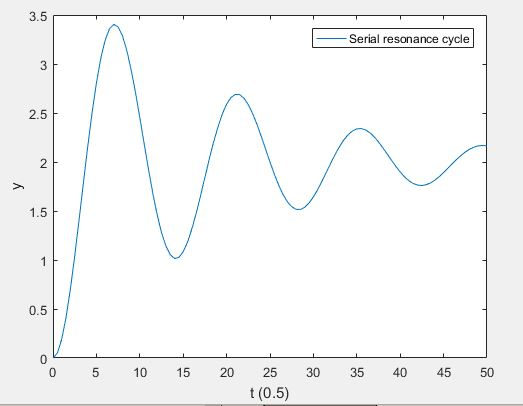
\includegraphics[scale=0.75]{\imageDir/sim_resonance_0.JPG}
\caption{Simulation 1 mit R1=1 , R2=2 , C=1 , L=2.5, U=1}
\label{fig:sim-resonance-01}
\end{figure}

\begin{figure}[h]
\centering
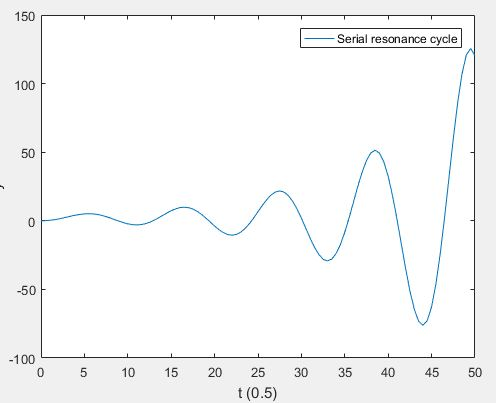
\includegraphics[scale=0.75]{\imageDir/sim_resonance_1.JPG}
\caption{Simulation 1 mit R1=1 , R2=2 , C=1 , L=1.5, U=1}
\label{fig:sim-resonance-01}
\end{figure}
\ \newpage

\begin{figure}[h]
\centering
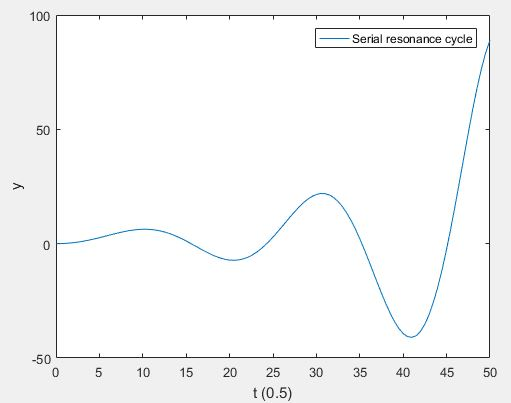
\includegraphics[scale=0.75]{\imageDir/sim_resonance_2.JPG}
\caption{Simulation 1 mit R1=1 , R2=2 , C=2 , L=2.5, U=1}
\label{fig:sim-resonance-01}
\end{figure}

\begin{figure}[h]
\centering
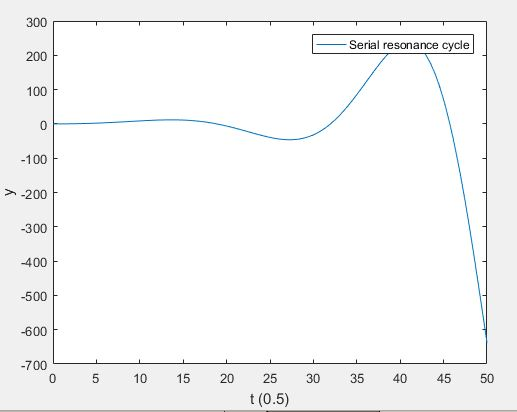
\includegraphics[scale=0.75]{\imageDir/sim_resonance_3.JPG}
\caption{Simulation 1 mit R1=1 , R2=2 , C=3 , L=2.5, U=1}
\label{fig:sim-resonance-01}
\end{figure}
\newpage

\section{Theorie der Kontinuierlichen Modellierung}
Dieser Abschnitt beschäftigt sich mit der Aufgabenstellung 3 der ersten Übung.
\subsection{3a Beschreibung der A,B,C Methode}
Dieser Abschnitt beschäftigt sich mit der Beschreibung der $A, B, C$ Methode.
\newline
\newline
Die $A, B, C$ Normalform verwendet die Matrizen $A, B$ und $C$, welche die Vektoren sind, mit denen die Eingangs-, die Ausgangs- und die Zustandsvariablen beeinflusst werden. 
\newline
\newline
\textbf{$A$-Matrix} ist der Vektor, der die gegenseitige Beeinflussung der inneren Zustandsvariablen beschreibt. Die $A$-Matrix hat so viele Spalten wie es innere Zustände gibt, die in der $X(0)$-Matrix durch die Anzahl der Zeilen gegeben ist.
\newline
\newline
$
A = \begin{bmatrix}
	\frac{R_{1}}{L} & -\frac{1}{L} \\[0.3em]
    \frac{1}{C}     & -\frac{1}{C*R_{2}} \\[0.3em]
\end{bmatrix}
X(0) =
\begin{bmatrix}
	1  \\[0.3em]
    10 \\[0.3em]
\end{bmatrix} 
$
\newline
\newline
\newline
\textbf{$B$-Matrix} ist der Vektor, der die Beeinflussung der Eingangsvariablen beschreibt. Die $B$-Matrix hat so viele Spalten wie es Eingangsvariablen gibt, die in der $U(t)$-Matrix durch die Anzahl der Zeilen gegeben ist.
\newline
\newline
$
B = \begin{bmatrix}
	\frac{R_{1}}{L} \\[0.3em]
	0
\end{bmatrix}
U(t) =
\begin{bmatrix}
	1  \\[0.3em]
\end{bmatrix} 
$
\newline
\newline
\newline
\textbf{$C$-Matrix} ist der Vektor, der definiert wird, je nachdem welchen Output man erhalten will. Die $C$-Matrix wird in der Ausgangsgleichung $y(t) = C * X(t)$ verwendet. Die Anzahl der Spalten ergibt sich aus der Anzahl der Zeilen der Ausgangsmatrix, die angibt wie viele Ausgangsvariablen es gibt. Die Werte $0$ und $1$ in der $C$-Matrix werden verwendet um die einzelnen Ausgangsvariabeln bei der Betrachtung miteinzubeziehen oder auszuschließen.
\newline
\newline
$
C
*
X(t)
$
;
$
\begin{bmatrix}
	1 & 0\\[0.3em]
\end{bmatrix}
*
\begin{bmatrix}
	i(t)  \\[0.3em]
	y(t)
\end{bmatrix}$
\hspace{1mm}
$|$
\hspace{1mm}
$
\begin{bmatrix}
	0 & 1\\[0.3em]
\end{bmatrix}
*
\begin{bmatrix}
	i(t)  \\[0.3em]
	y(t)
\end{bmatrix} 
$
\hspace{1mm}
$|$
\hspace{1mm}
$
\begin{bmatrix}
	1 & 0\\[0.3em]
	0 & 1\\[0.3em]
\end{bmatrix}
*
\begin{bmatrix}
	i(t)  \\[0.3em]
	y(t)
\end{bmatrix} 
$
\newline
\newline
\newline
Hat man sein System auf die $A, B, C$ Normalform gebracht, kann man die einzelnen Werte zum Zeitpunkt $t$ mit dem Integral ausrechnen, das sich durch die Umformung der Eingans- und Ausgangsgleichung ergibt, wenn es sich um eine lineare Gleichung handelt und wenn der Zustand $X(0)$ bekannt ist. Die aufgestellte Eingangs- und Ausgangsgleichung beschreiben das System, die in einer Simulationssoftware dazu verwendet werden kann, um das System über die Zeit $t$ zu simulieren. 
\newline
\newline
Diese mathematische Beschreibung zeigt, die Zusammenhänge und Beeinflussung der Variablen innerhalb des Systems. Mit der $A, B, C$ Normalform, kann die Veränderung eines Zustands im System zum Zeitpunkt $t$ berechnet werden. Die Berechnung kann auch exakt erfolgen, wenn das System mit einer linearen Differenzialgleichung beschrieben ist.
\newline
\newline
Bei einer Simulation kann neben der Annäherung auch die exakte Simulation eines Systems erfolgen, das mit der Eingangs- und Ausgangsgleichung in $A, B, C$ Normalform beschrieben ist. Ohne die Berechnungen mit den Gleichungen der $A, B, C$ Normalform kann keine Simulation eines Systems erfolgen, das durch diese Gleichungen beschrieben ist.
\newpage
\subsection{3b Zusammenhang der Formeln der A, B, C Methode}
Dieser Abschnitt beschäftigt sich mit der Beschreibung des Zusammenhangs der Formeln der $A, B, C$ Methode.
\newline
\newline
Ein System in der $A, B, C$ Normalform, kann mit den Eingans- und Ausgangsgleichungen die Simulationen über die Zeit $T$ erstellen werden. Die aufgestellten Differenzialgleichungen beschreiben das zu testende System, wobei die Vektoren $A, B, C$ die Beeinflussung der Eingangs-, Ausgangs- und inneren Zustandsvariablen beschreiben. Das Integral kann dazu verwendet werden, um zu einem Zeitpunkt $t$ den exakten Zustand eines Systems zu berechnen, wenn die aufgestellte Differenzialgleichung eine lineare Differenzialgleichung ist. 

\end{document}